%!TEX TS-program = xelatex
%!TEX encoding = UTF-8 Unicode
\documentclass[slides,english,compress]{beamer}

\usetheme{Boadilla}%soft colors, pretty nice
%%%%%%%%%%%%%%%%%%%%%%%%%%%%%%%%%%%%%%%%%%%%%
%Below to get rid of headers and footers on all pages
\setbeamertemplate{headline}{}
%gets rid of bottom navigation bars
\setbeamertemplate{footline}[frame number]{}

%gets rid of bottom navigation symbols
\setbeamertemplate{navigation symbols}{}

%gets rid of footer
%will override 'frame number' instruction above
%comment out to revert to previous/default definitions
\setbeamertemplate{footline}{}
%%%%%%%%%%%%%%%%%%%%%%%%%%%%%%%%%%%%%%%%%%%%%%
%\usepackage{pgfpages}
\usepackage{eurosym}
\usepackage{makeidx}
\usepackage{amsthm,amsmath,amssymb,amsfonts}
\usepackage{polyglossia} 
%\usepackage{fontspec}
\usepackage{xunicode}
\usepackage{xltxtra} 
\synctex=1

%\usepackage{xltxtra}

%\usepackage{geometry}

\usepackage{subfig}
\usepackage[normalem]{ulem}

\usepackage{graphics, graphicx}
\usepackage{hyperref}

\usepackage{enumerate}

\usepackage{tikz}
\usetikzlibrary{calc}
\usetikzlibrary{intersections}
\colorlet{examplefill}{blue!10}
\makeatletter%This is to find the coordinates of a node
\newcommand{\gettikzxy}[3]{%
  \tikz@scan@one@point\pgfutil@firstofone#1\relax
  \edef#2{\the\pgf@x}%
  \edef#3{\the\pgf@y}%
}
\makeatother


\newcommand{\tikzmark}[1]{\tikz[overlay,remember picture] \node (#1) {};}
\newcommand{\DrawBox}[1][]{%
    \tikz[overlay,remember picture]{
    \draw[red,#1]
      ($(left)+(-0.1em,0.9em)$) rectangle
      ($(right)+(0.1em,-0.3em)$);}
}

\usepackage[all]{xy}
%\usepackage{xcolor}
\usepackage{color,soul} 
\definecolor{lightblue}{rgb}{.90,.95,1}
\sethlcolor{lightblue}
%\selectcolormodel{rgb}
%\convertcolorsUfalse     


\usepackage{pgfpages} % for multiple-screen presentations
%\usepackage{embedfile}
%\IfFileExists{\jobname.nav}{\embedfile{\jobname.nav}}{}
%\embedfile{\jobname.tex}
%\setbeameroption{show only notes}
%\setbeameroption{show notes on second screen}
% \setbeameroption{second mode text on second screen=left} % might not let animations work

\makeatletter
\def\beamer@framenotesbegin{% at beginning of slide
  \gdef\beamer@noteitems{}%
  \gdef\beamer@notes{{}}% used to be totally empty.
}
\makeatother

\newtheorem{proposition}{Proposition}
%\setbeamertemplate{navigation symbols}{}
%\setbeamertemplate{blocks}[rounded][shadow=true]

%\mode<presentation>

%\includeonlyframes{current} %to be deleted after the presentation is complete: current speeds up compilation




%\useheadtemplate{
%\vbox{
%  \vskip3pt
 % \insertsectionnavigationhorizontal{\textwidth}{}{}
 % \vskip1pt
  %\insertvrule{0.4pt}{structure!50}
 % \vskip3pt
  %\insertsubsectionnavigationhorizontal{\textwidth}{}{}
 % \vskip1pt
  %\insertvrule{0.4pt}{structure!50}}
%}

\title{Learning Within or Outside Firms: Labor Market Frictions and Entrepreneurship }

\author{
Andrea Canidio\thanks{INSEAD} \and Patrick Legros\thanks{Northeastern U., Université libre de Bruxelles (ECARES), and CEPR} }


\date{MIT Org Lunch Seminar\\12 April 2017}

\begin{document}

\frame[plain]{\titlepage}

%\setbeamertemplate{footline}[frame number]

\section{Introduction}

\begin{frame}
  \frametitle{}
 Extended revision of \\

 \vspace{1cm}
 \textcolor{blue}{``The Value of Entrepreneurial Failures: Task Allocation and Career Concerns''} (CEPR 2016)
\end{frame}
%%%%%%%%%%%%%%%%%%%%%%%%%%%%%%%%%%%%%%%%%%%%%%%%%%%%%%%%%%%%
\begin{frame}
	\frametitle{The Labor Market, Firms and Motives for Entrepreneurship}

\onslide<1-2>{\begin{block}{If individuals get job offers rarely:}
\begin{itemize}
	\item Poaching by competitors is a rare event. Firms have incentives to make investments in learning their workers' productivity that have a long-term benefit, even if it comes at the expense of short-term profits.
	\item \structure{Motives for entrepreneurship:} no job offer or a better project than what is available by working for a firm. Fear of not finding a job later. 
\end{itemize}	
\end{block}
}
%\only<1>{Gottlieb, Townsend, Xu (2016)}
\onslide<2>{\begin{block}{If agents get job offers easily:}
	\begin{itemize}
	\item Job poaching: learning about long-term benefits is discouraged in firms.
	\item Entrepreneurs have a \structure{new motive for entrepreneurship:} \alert{learning their long-run productivity}
	\end{itemize}
\end{block}	
}	
\end{frame}
%%%%%%%%%%%%%%%%%%%%%%%%%%%%%%%%%%%%%%%%%%%%%%%%%%%%%%%%%%%
\begin{frame}
	\frametitle{}
We show how this tradeoff between \alert{short-termism} by firms and the \alert{learning motive for entrepreneurship} has consequences for:
	\vspace{0.5cm}
	
	\begin{itemize} \setlength\itemsep{0.5em}
		\item The career path of individuals: in-and-out of entrepreneurship of in-and-out of employment. %The probability of being a serial entrepreneur, etc.
		\item The wage difference of previous entrepreneurs and previous workers (value of failures).
	\end{itemize}
\end{frame}

%%%%%%%%%%%%%%%%%%%%%%%%%%%%%%%%%%%%%%%%
\begin{frame}
	\frametitle{Literature}
	
\only<1>{
\begin{block}{Employment \& Entrepreneurship}	\begin{itemize}
		\item Banerjee-Newman (1993); financial imperfections shape firms' organizations and  the choice between self-employment, employment and firm creation. No learning motive. 
		\item Vereshchagina and Hopenayn (2009): return to entrepreneurship is uncertain but can be learned (nothing to learn in firms).
		\item Manso (2016); confirms experimentation view, assumes that failed entrepreneurs can find easily an employment contract.
	\end{itemize}	
\end{block}	
}
\only<2>{
\begin{block}{Choices of firms and entrepreneurs}	
	\begin{itemize}
				\item Hellmann (2007); employees becoming entrepreneurs, because firms are focused on their core activities and discourage innovation  (no learning).
		\item De Bettignies and Chemla (2008); corporate venturing and competition for talented managers.
	\end{itemize}	
\end{block}	
}

\only<3>{
\begin{block}{Talent discovery}
	\begin{itemize}
		\item \emph{Information accumulation model}. MacDonald (1982a,b): task assignment when agents have different comparative advantages; frictionless labor market and no entrepreneurship.  Also, Gibbons-Waldman (1999, 2004), career path \emph{within} a firm.
		\item Papageorgiou (2013); labor market frictions and talent discovery. Firms = one task; no entrepreneurship; individuals must move between firms to learn. (Also  Eeckhout and Weng 2009; no labor market frictions.)
		\item Postarino (2013), structural estimation of learning by firms via task assignment. xAntonovics and Golan (2012); information revealed in different jobs.
	\end{itemize}
\end{block}
}

\only<4>{
\begin{block}{Value of failures 1}
	\begin{itemize}
		\item Gromb and Scharstein (2002); replace failed managers by failed entrepreneurs
		\item Landier (2005); in general stigma failed entrepreneurs.
		\item Other views:
	\begin{quote}
		``Failure is only the opportunity to begin again more intelligently'' (Henry Ford)
	\end{quote}	
	\begin{quote}
		``Failure Chronicles'' (HBReview 2011)
	\end{quote}
	\begin{quote}
		``Adapt: Why Success Always Starts with Failure'' (Tim Harford)
	\end{quote}
	\end{itemize}
\end{block}
}

\only<5>{
\begin{block}{Value of failures 2}
	\begin{itemize}
		\item Gompers-Kovner-Lerner-Scharstein (2010): failed entrepreneurs are marginally \structure{more likely} to succeed than first time entrepreneurs
		\item Hamilton (2000; table 6): entrepreneurs who re-enter the labor market earn \structure{higher wages} than comparable workers. (Also Evans-Leighton 1990, Daly 2015.)
		\pause
		\item Gottschalk-Greene-H\"ower-M\"uller (2014); failed entrepreneurs \alert{less likely} to succeed than first time entrepreneurs.
		\item Baptista-Lima-Preto (2012); wage of former entrepreneurs is \alert{lower} than wage of former workers
	\end{itemize}
\end{block}
}


\end{frame}
%%%%%%%%%%%%%%%%%%%%%%%%%%%%%%%%%%%%%%%%
\section{Model}

\begin{frame}
	\frametitle{}
	\begin{center}%[<+->]
		\Huge Model 
	\end{center}
\end{frame}
%%%%%%%%%%%%%%%%%%%%%%%%%%%%%%%%%%%%%%%%%
\begin{frame}
	\frametitle{Agents and firms}
	\begin{itemize}
		\item Two periods
		\item Free entry of firms in each period
		\item Continuum of agents who live for two periods
		\item Agent type is $\theta\in\{l,h\}$
		\item Common initial belief: $\mbox{pr}\{\theta=h\}=p_1$
	\end{itemize}
\end{frame}
%%%%%%%%%%%%%%%%%%%%%%%%%%%%%%%%%%%%%%%%
\begin{frame}
	\frametitle{Production}
	\begin{itemize}
		\item A project succeeds or fails; if fails, it brings a monetary payoff of zero
		\item Each period, same off-the-shelf project $K_t$ for \alert{all firms}; \alert{$K_t\sim U[0,2]$}, i.i.d..
		\item Each period, \alert{each agent} draws a project $k_t$; \alert{$k_t\sim U[0, \alert{\lambda}K_t]$}, $\lambda\geq 1$. 
		\item Two ways to produce, \alert{task} $\tau\in\{A,B\}$ 
	\end{itemize}

\end{frame}
%%%%%%%%%%%%%%%%%%%%%%%%%%%%%%%%%%%%%%%%
\begin{frame}
	\frametitle{Returns to tasks}
		\[  
  \begin{array}{  c |c  c }
  \tau\backslash\theta & l & h \\
  \hline
 B & l_B & h_B \\
A & l_A & h_A 
\end{array}
\]
\only<2>{\begin{block}{Assumptions}
	\begin{enumerate}
		\item High types are more productive: $\max(h_A,h_B) \geq \max(l_A,l_B)$
		\item Comparative advantages: $h_A-h_B>0, l_B-l_A>0$
	\end{enumerate}
\end{block}
}
\only<3>{
\begin{itemize}
\item(\textbf{Vertical talent}) If $h_B \geq l_B$ the probabilities of success at both tasks are at least as large for type $h$ than type $l$.\item (\textbf{Horizontal talent}) When $h_B<l_B$, high type agents have a larger probability of success only if assigned to the advanced task $A$. 
\end{itemize}
}
\end{frame}
%%%%%%%%%%%%%%%%%%%%%%%%%%%%%%%%%%%%%%%%
\begin{frame}
	\frametitle{}
	\begin{figure}[h!]
\centering
	\begin{tikzpicture}[scale=0.8]
	\draw [dashed](0,0) node[below]{$\theta=l$}-- (0,6);
	\draw [dashed] (5,0) node[below]{$\theta=h$} -- (5,6);
	\draw[fill=green] (5,6) circle(0.3) node[right=1em]{$h_A$};
	\draw[fill=red] (5,3) circle(0.3) node[right=1em]{$h_B$};
	\only<2>{
	\draw[fill=green] (0,2.5) circle(0.3) node[left=1em]{$l_B$};
	\draw[fill=red] (0,1) circle(0.3) node[left=1em]{$l_A$};
	\draw (2.5,3) node[red,thick]{Vertical talent};
	}
	\only<3>{
	\draw[fill=green] (0,4) circle(0.3) node[left=1em]{$l_B$};
	\draw[fill=red] (0,1) circle(0.3) node[left=1em]{$l_A$};
	\draw (2.5,3) node[red,thick]{Horizontal talent};
	}
	\only<4>{
	\draw[fill=green] (0,4.5) circle(0.3) node[left=1em]{$l_B$};
	\draw[fill=red] (0,3.5) circle(0.3) node[left=1em]{$l_A$};
	\draw (2.5,3) node[red,thick]{Horizontal talent};
	}
	\end{tikzpicture}
\end{figure}
\end{frame}
%%%%%%%%%%%%%%%%%%%%%%%%%%%%%%%%%%%%%%%%
\begin{frame}
	\frametitle{Contract offers}
	A contract by a firm is \alert{$(f,b)$}, $f$ a fixed payment, $b$ a share of the return.
	
\begin{block}{Assumptions}	
	\begin{enumerate}[(i)]
\item \alert{Contract incompleteness:} the bonus is strictly bounded above by the monetary return of the firm, that is \alert{$b\leq \beta$} where $\beta<1$.
\item \alert{Residual right to decide on task allocation:} Task allocation within firms is observable but not contractible.
\item No long-term contract (...extension)
\end{enumerate}  
\end{block}

\end{frame}
%%%%%%%%%%%%%%%%%%%%%%%%%%%%%%%%%%%%%%%%
\begin{frame}
	\frametitle{Labor market frictions}

\begin{block}{Probability of getting offers}
	With probability $1-\alpha$ an agent receives no offer from firms, and with probability \alert{$\alpha$} he receives at least two offers
\end{block}
%
\vspace{0.5cm}
\textcolor{gray}{$\rightarrow$ Ridder and Berg 2003 estimates of job offer arrival rates in EU, US, and other countries}
\end{frame}
%%%%%%%%%%%%%%%%%%%%%%%%%%%%%%%%%%%%%%%%
\begin{frame}
	\frametitle{Timing}
	  \begin{figure}[h!]
\centering
	\begin{tikzpicture}[scale=0.7, every node/.style={scale=0.4}]
    \tikzstyle{every node} = [align=center]
	\draw[->] (-4,0)--(12,0) node[left=-5pt,below]{};
	\foreach \x in {0,3,6,9,12}
	\draw (\x-2,-10pt) -- (\x-2,10pt);
	
	\draw (-2,10pt) node[fill=examplefill, text width=2cm, above]{All firms draw project $K_t$. Each individual draws a project $k_t\leq \lambda K_t$ };
	\draw (1,-10pt)  node[fill=examplefill,text width=2cm,below]{Contracts are offered};
    \draw (4,10pt) node[fill=examplefill,text width=2cm,above]{Agents choose\\ entrepreneur\\ or employment};
	\draw (7,-10pt) node[fill=examplefill, text width=2cm,below]{ Task allocation\\ $\tau_t$ is chosen};
	\draw (10,10pt) node[fill=examplefill,text width=2cm, above]{Success or\\ failure realized};
	\end{tikzpicture}
	\caption{timing withing period $t=1,2$}
\end{figure}
\end{frame}
%%%%%%%%%%%%%%%%%%%%%%%%%%%%%%%%%%%%%%%%
\section{Static vs dynamic efficiency}
\begin{frame}
	\frametitle{}
	\begin{center}%[<+->]
		\Large Static vs Dynamic Efficiency:\\ the Informativeness of Task Allocation
	\end{center}
\end{frame}
%%%%%%%%%%%%%%%%%%%%%%%%%%%%%%%%%%%%%%%%
\begin{frame}
	\frametitle{}
\only<1>{	For any prior belief  $p_t$  that the individual is of type $h$, the probability that there is a success in a given period is: 
\begin{equation}\label{eq:pr of success}
\pi(\tau_t,p_t)\equiv \begin{cases}
(1-p_t)\cdot l_A + p_t \cdot h_A  &\mbox{if } \tau_t=A\\
(1-p_t) \cdot l_B + p_t \cdot h_B  &\mbox{if } \tau_t=B.
\end{cases}\notag
\end{equation}
}
%

\only<2-3>{It follows that the probability of success in the current period is maximized by assigning the agent to task $B$ if and only if $p_t$ is smaller than the cutoff value
\begin{equation*}
q^* \equiv \left(1+ \frac{h_A-h_B}{l_B-l_A} \right)^{-1}.
\end{equation*}
}
\only<3>{
Call  \alert{$\pi^M(p_t)$} the maximum probability of success in a given period, defined as
\begin{align}\label{maxp}
\pi^M(p_t)&\equiv\max_{\tau_t}\pi(\tau_t,p_t)
=\begin{cases} 
(1-p_t) l_B + p_t h_B &\mbox{if } p_t \leq q^*\\
(1-p_t) l_A + p_t h_A & \mbox{if } p_t \geq q^* ,
\end{cases}\notag
\end{align}

}
\end{frame}
%%%%%%%%%%%%%%%%%%%%%%%%%%%%%%%%%%%%%%%%
%%%%%
%   
% Two cases vertical and horizontal talent‰               
%    
%%%%%
\begin{frame}
	\frametitle{}

\begin{figure}[h!]
    \centering
    \subfloat[Vertical case: $h_B>l_B$]{%
 \begin{tikzpicture}[scale=0.6,transform shape]
\draw[->] (0,0) -- (9,0)node[below]{$p_t$};
\draw [->](0,0)--(0,6) node[left]{$\pi^M(p_t)$};
%%%%

\draw (0,5)  node[left]{$h_A$};
\draw (0,3.5) node[left]{$h_B$};
\draw (0,2) coordinate (B) node[left]{$l_B$};
\draw (0,1) coordinate (A) node[left]{$l_A$};
%
\draw[gray] (A)--(7,5) coordinate (C) node[right]{$A$};
\draw [gray] (B)--(7,3.5) coordinate (D) node[right]{$B$};
%Find intersection
 \fill[red] (intersection cs:
    first line={(A)--(C)},
    second line={(B)--(D)}) coordinate (I) circle (2pt);
%%%Projection
\draw[dotted] (I)--($(0,0)!(I)!(5,0)$) node[below]{$q^*$};
\draw[very thick,blue] (B)--(I)--(C);
\end{tikzpicture}}
%%%%%%%%%
    \centering
    \subfloat[Horizontal case: $h_B<l_B$]{%
 \begin{tikzpicture}[scale=0.6,transform shape]
\draw[->] (0,0) -- (9,0)node[below]{$p$};
\draw [->](0,0)--(0,6) node[left]{$\pi^M(p)$};
%%%%
\draw (0,5)  node[left]{$h_A$};
\draw (0,3.5) coordinate (B) node[left]{$l_B$};
\draw (0,2)  node[left]{$h_B$};
\draw (0,1) coordinate (A) node[left]{$l_A$};
%
\draw[gray] (A)--(7,5) coordinate (C) node[right]{$A$};
\draw [gray] (B)--(7,2) coordinate (D)node[right]{$B$};
%Find intersection
 \fill[red] (intersection cs:
    first line={(A)--(C)},
    second line={(B)--(D)}) coordinate (I) circle (2pt);
%%%Projection
\draw[dotted] (I)--($(0,0)!(I)!(5,0)$) node[below]{$q^*$};
\draw[very thick,blue] (B)--(I)--(C);
\end{tikzpicture}}
%%%%%%%%%%%%%%%
  \caption{Maximum probability of success as a function of belief $p_t$.}
  \label{fig: success 2}
\end{figure}
\end{frame}
%%%%%%%%%%%%%%%%%%%%%%%%%%%%%%%%%%%%%%%%
\begin{frame}
	\frametitle{}
Denote \[\sigma_1(\tau_1) \equiv \pi(\tau_1,p_1),\] 

\begin{block}{Assumption}
\structure{$p_1<q^*$: task $B$ maximizes the initial probability of success, that is $\sigma_1(B)>\sigma_1(A)$.}
\end{block}

\vspace{1cm}

We are interested in establishing the conditions under which $\tau_1=A$ maximizes the \alert{period-2 expected probability of success}. Hence, whether \structure{$A$ is more informative than $B$.}
\end{frame}
%%%%%%%%%%%%%%%%%%%%%%%%%%%%%%%%%%%%%%%%
\begin{frame}[label=sigma2]
	\frametitle{$\sigma_2(A)>\sigma_2(B)$?}

Period 2 expected probability of success from period 1's perspective:
\begin{equation*}
\alert{\sigma_2(\tau_1) \equiv \mathbb E_{s_1\in\{0,1\}}\pi^M (p_2(\tau_1,s_1))},
\end{equation*}

\vspace{0.5cm}

\only<2>{Where $p_2(\tau_1,s_1)$ is the posterior belief at time $2$ given period $1$ task allocation and success or failure:
	\[p_2(\tau_1,s_1)\equiv \begin{cases} 
\left(\frac{1-p_1}{p_1}\frac{l_{\tau_1}}{h_{\tau_1}}+1\right)^{-1} &\mbox{ if } s_1=1\\
\left(\frac{1-p_1}{p_1}\frac{1-l_{\tau_1}}{1-h_{\tau_1}}+1\right)^{-1} &\mbox{ if } s_1=0
\end{cases}
\]
}
\only<3>{Since
\begin{equation*}
\mathbb E_{s_1\in\{0,1\}}\pi (\tau_1,p_2(\tau_1,s_1)) p_2(\tau_1,s_1)=p_1.
\end{equation*}
and $\pi^M(p_2)$ is convex (piece-wise linear) in $p_2$, with a kink at $q^*$
}

\only<4>{A necessary condition for $\sigma_2(A)>\sigma_2(B)$ is that $p_2(A,1)>q^*$, that is 
\[p_1\geq q_A\equiv \left(1+\frac{h_A}{l_A}\frac{h_A-h_B}{l_B-l_A}\right)^{-1}\]
and a sufficient condition is that $(p_2(A,s_1))$ is a MPS of $(p_2(B,s_1))$.

}

\only<5>{MPS holds automatically in the vertical talent case, hence the NSC is $p_1\geq q_A$. MPS does not hold automatically in the horizontal talent case, and stronger conditions may have to be imposed. 
\hyperlink{mps}{\beamergotobutton{mps}}
}
\end{frame}
%%%%%%%%%%%%%%%%%%%%%%%%%%%%%%%%%%%%%%%%
\begin{frame}
	\frametitle{Example}
	
			\[  
  \begin{array}{  c |c  c }
  \tau\backslash\theta & l & h \\
  \hline
 B & 0.6 & 0.4 \\
A & 0.1 & 0.9 
\end{array}
\]
	\begin{figure}[h!]
\centering
	\begin{tikzpicture}[scale=0.8,transform shape]
	\draw [->](0,0) node[left=2em,below]{$0$}-- (10,0) node[right,below]{$p_1$};
	\draw [->] (0,0) -- (0,4) node[left]{variations};
    \draw[very thick, blue,name path=line1] (0,0)--(1,0)node[below,black]{$q_A=0.1$}--(4.5,1.4)--(6,1.5)node[right]{$\sigma_2(A)-\sigma_2(B)$};
   \draw (6,0)node[below]{$q^*=0.5$};
 
    \draw[gray!20](0,0)--(6,1.5);
        \draw [orange, very thick,name path=line2] (6,0)--(1,3.5) node[right=1em]{$\sigma_1(B)-\sigma_1(A)$};
      \path [name intersections={of=line1 and line2,by=E}];
%\node [fill=red,circle,inner sep=1pt] at (E) {};
\gettikzxy{(E)}{\ex}{\ey};
%\pause
%\draw[dotted,red,thick] (E) --(\ex,-1) node[right]{conflict} node[left]{no conflict};
	\end{tikzpicture}
\end{figure}
%Each variation shoudl be weighted by the expected returns in first vs second period
\end{frame}
%%%%%%%%%%%%%%%%%%%%%%%%%%%%%%%%%%%%%%%%
\begin{frame}
	\frametitle{Failures: Good News or Bad News?}
	
	\begin{block}{Lemma}\begin{enumerate}[(i)]\setlength\itemsep{0em}
\item In the vertical-talent case failures are always bad news, that is,  \alert{$\pi^M(p_2(\tau_1,0))<\pi^M(p_1)$} for all $\tau_1\in \{A,B\}$.
\item In the horizontal-talent case, failures at task $A$ are always good news, that is, \alert{$\pi^M(p_2(A,0))>\pi^M(p_1)$}. There is a threshold $q_B$ such that failures at task $B$ are bad news for $p_1<q_B$ and good news for $p_1>q_B$.
\end{enumerate}
\end{block}
	
\end{frame}
%%%%%%%%%%%%%%%%%%%%%%%%%%%%%%%%%%%%%%%%
\section{Equilibrium choices}
\begin{frame}
	\frametitle{}
	\begin{center}%[<+->]
		\Large Equilibrium Choices
	\end{center}
\end{frame}
%%%%%%%%%%%%%%%%%%%%%%%%%%%%%%%%%%%%%%%%%%%%%%
\begin{frame}
	\frametitle{Period 2 expected payoff of an entrepreneur}
\begin{block}{}
	\structure{Get an offer ($\alpha$):}
%
	\[\sigma_2(\tau_1) \cdot \mathbb E[\max\{k_2,K_2\}]=\sigma_2(\tau_1) \cdot \frac{1}{2} \left( \lambda + \frac{1}{\lambda} \right)
	\]
\structure{Does not get an offer ($1-\alpha$):} (forced to stay an entrepreneur) \[\sigma_2(\tau_1)\mathbb E[k_2]=\sigma_2(\tau_1)\frac{\lambda}{2}.\]
\end{block}	
\pause
Entrepreneur chooses $\tau_1$:
\begin{align*} 
\max_{\tau_1}\sigma_1(\tau_1) k_1+  \sigma_2(\tau_1)  \left(  \frac{\alpha}{2} \left( \lambda + \frac{1}{\lambda} \right) + (1-\alpha) \frac{\lambda}{2} \right).
\end{align*}
\end{frame}
%%%%%%%%%%%%%%%%%%%%%%%%%%%%%%%%%%%%%%%%
\begin{frame}
	\frametitle{Period 1: Entrepreneur}


Optimal to choose $\tau_1=A$ whenever
\begin{align*}\label{eq: optimal entrepreneur}
k_1\leq \alert{k^A(\alpha)} \equiv   \frac{\alpha+\lambda^2}{2\lambda}\times\frac{\sigma_2(A)-\sigma_2(B)}{\sigma_1(B)-\sigma_1(A)},
\end{align*}

\vspace{1cm}
\only<2>{
Expected payoff of a period 1 entrepreneur:
\[
\alert{W^E(k_1,\alpha)}=\begin{cases}
\sigma_1(A) k_1+  \sigma_2(A)  \frac{\alpha+\lambda^2}{2\lambda} &\mbox{if } k_1\leq k^A(\alpha) \\
\sigma_1(B) k_1+  \sigma_2(B)  \frac{\alpha+\lambda^2}{2\lambda} &\mbox{if } k_1 > k^A(\alpha), 
\end{cases}
\]
}
\end{frame}
%%%%%%%%%%%%%%%%%%%%%%%%%%%%%%%%%%%%%%%%
\begin{frame}
	\frametitle{Period 1: Worker}
Even if firms compete for workers at $t=1$, workers care about the (not contractible) task allocation that will be chosen by firms since it affects their period 2 expected payoff:
\only<2>{
\begin{block}{}
\structure{Get an offer ($\alpha$):}
	\[\sigma_2(\tau_1) \cdot \mathbb E[\max\{k_2,K_2\}]=\sigma_2(\tau_1) \cdot \frac{1}{2} \left( \lambda + \frac{1}{\lambda} \right)
	\]
\structure{Does not get an offer ($1-\alpha$):} (split the surplus with firm) \[\sigma_2(\tau_1)\mathbb {E}\left[k_2+\frac{1}{2}\max\{K_2-k_2,0\}\right]= \sigma_2(\tau_1) \frac{5}{4 \lambda};\]
	{\centering \alert{the firm gets $\sigma_2(\tau_1) \frac{1}{4 \lambda}$.}}
\end{block}	
}	
\end{frame}
%%%%%%%%%%%%%%%%%%%%%%%%%%%%%%%%%%%%%%%%
\begin{frame}
	\frametitle{}
	
\begin{block}{Commitment value of bonuses}
		\begin{itemize}
			\item 
		Since  $b\leq\beta K_1$,  the firm can commit to implement task $A$ in the first period if $( \sigma_1(B)- \sigma_1(A))(1-\beta)K_1\leq(\sigma_2(A)-\sigma_2(B))\frac{1-\alpha}{4\lambda} $, that is when 

\begin{equation*}
K_1\leq K^A(\alpha)\equiv   \frac{1-\alpha}{4 \lambda (1-\beta) }\times \frac{ \sigma_2(A)- \sigma_2(B)}{ \sigma_1(B)- \sigma_1(A)}.
\end{equation*}

\item Since $b\geq 0$, firm can commit to implement task $B$ when
$(\sigma_1(B)-\sigma_1(A))K_1 \geq (\sigma_2(A)-\sigma_2(B))\frac{1-\alpha}{4\lambda}$, that is when
\begin{equation*}%\label{minKB}
K_1\geq K^B(\alpha)\equiv \frac{1-\alpha}{4 \lambda } \times \frac{ \sigma_2(A)- \sigma_2(B)}{ \sigma_1(B)- \sigma_1(A)} .
\end{equation*}
		\end{itemize}
		
\end{block}

\end{frame}
%%%%%%%%%%%%%%%%%%%%%%%%%%%%%%%%%%%%%%%%
\begin{frame}
	\frametitle{}

Best payoff a firm can offer at $t=1$ is subject to the firm-IC constraint of task allocation in period 1:
\begin{align*}
W^F(K_1,\alpha) \equiv \begin{cases}
&\max_{\tau_1=A,B} \sigma_1(\tau_1)K_1+\sigma_2(\tau_1)\frac{1+\lambda^2}{2\lambda}\\
& \hspace{1cm} \tau_1=A\Rightarrow K_1\leq K^A(\alpha)\\
& \hspace{1cm} \tau_1=B\Rightarrow K_1\geq K^B(\alpha).
\end{cases}
\end{align*}


\vspace{0.5cm}
\only<2>{
\textcolor{gray}{Note that $\sigma_1(\tau_1)K_1+\sigma_2(\tau_1)\frac{\lambda^2+1}{2\lambda}$ is both the total output generated within a firm, and the total expected output generated by an entrepreneur with project $k_1=K_1$, in the absence of labor market frictions (that is, when $\alpha=1$).   It follows that the two period total output generated within firms is maximized by task $A$ if, and only if, $ K_1\leq  k^A(1)$}}
\only<3>{
\structure{In a competitive equilibrium, firms choose contracts that implement task $\tau_1=A$ if $K_1\leq \min\left\lbrace K^A(\alpha), k^A(1) \right \rbrace $ and task $\tau_1=B$ otherwise.}
}
\end{frame}
%%%%%%%%%%%%%%%%%%%%%%%%%%%%%%%%%%%%%%%%
\begin{frame}
	\frametitle{}
\begin{lemma}
\begin{enumerate}[(i)]\setlength\itemsep{0.5em}
\item  Whenever $K_1 \geq  k^A(1)$ or $K_1 \leq K^A(\alpha)$ the equilibrium task allocation maximizes the two-period total output.
\item \alert{Whenever $K_1 \in \left( K^A(\alpha), k^A(1) \right)$  the firm's task allocation is inefficient: the two-period total output is maximized by $\tau_1=A$ but firms implement $\tau_1=B$.}\end{enumerate}
\end{lemma}

\end{frame}
%%%%%%%%%%%%%%%%%%%%%%%%%%%%%%%%%%%%%%%%

\begin{frame}
	\frametitle{}
	\begin{center}%[<+->]
		\Large Two Regimes  
	\end{center}
\end{frame}

%%%%%%%%%%%%%%%%%%%%%%%%%%%%%%%%%%%%%%%%

\begin{frame}
	\frametitle{Second period wages: former entrepreneurs vs former workers}

\only<1>{As $\alpha$ increases, previous entrepreneurs are more likely to use $A$ while firms are more likely to use $B$, hence the second period wages of previous entrepreneurs increase while those of previous workers decrease in $\alpha$.
}

\only<2-3>{
\begin{block}{Proposition}\
%\item  The expected period 2 wage of a period 1 entrepreneur is increasing in $\alpha$.
%\item The expected period 2 wage of a period 1 worker is decreasing in $\alpha$.  
 There exists  $\alpha^*\in(0,1)$ such that the period 2 wage of a former entrepreneur is greater than the wage of a former worker if and only if $\alpha>\alpha^*$.
\end{block}
}
\vspace{1cm}


\only<3>{
\textcolor{gray}{$\rightarrow$ Hamilton 2000 and Baptista et al. 2012}
}
\end{frame}
%%%%%%%%%%%%%%%%%%%%%%%%%%%%%%%%%%%%%%%%

\begin{frame}
	\frametitle{Ex: Probabilities of entrepreneurship}
\begin{itemize}
	\item \structure{Necessity entrepreneurs:} agents who do not get wage offers
	\item \structure{Opportunity entrepreneurs:} agents who would prefer to be entrepreneurs independently of the task allocation used in firms (high $k_1$)
	\item \structure{Learning entrepreneurs:} choose entrepreneurship because firms implement task $\tau_1=B$ despite the fact that task $\tau_1=A$ maximizes the two period output.
\end{itemize}



\end{frame}

%%%%%%%%%%%%%%%%%%
%%%%%%%%%%%%%%%%%%%%%%%%%%%%%%%%%%%%%%%%%%%%%
\begin{frame}
	\frametitle{Large market frictions ($K^A(\alpha)>k^A(1)$): no learning entrepreneurs}
	\begin{figure}

\begin{tikzpicture}[thick, scale=1.4]
\draw [<->] (0,4) node[above]{Payoff} --  (0,0) -- (6.5,0);
\node [below] at (6.5,0) {$K_1,~k_1$};
%\draw[dotted] (0,1)--(6,4);
%\draw[dotted] (0,2)--(6,3.5);
\draw[] (0,2)--(4,3) node[midway, sloped, above] {task $A$ in firms};
\draw[] (4,3)--(6,4) node[midway, sloped, above] {task $B$ in firms};
\node[right] at (6,4) {$W^F(K_1,\alpha)$};
\draw[blue] (0,.6)--(2.8,1.3) node[midway, sloped, above] {task $A$ as entrepreneur};
\draw[blue] (2.8,1.3)--(6,2.9)  node[midway, sloped, above] {task $B$ as entrepreneur};
\node[right,blue] at (6,2.9) {$W^E(k_1,\alpha)$};

\only<1>{
\draw[dotted] (4,3)--(4,0);
\node[below] at (4,0) {$k^A(1)$};
\node[below] at (5.2,0) {$K^A(\alpha)$};
\draw[dotted] (2.8,1.3)--(2.8,0);
\node[below] at (2.8,0) {$k^A(\alpha)$};
}

%\draw[dotted] (0,.5)--(6,3.5);
%\draw[dotted] (0,1)--(6,2.5);
\only<2>{
\node[below, red] at (.7,0) {$A$};
\draw[dashed,red,->,very thick] (.7,0)--(.7,2.17)--(4.51,2.17)--(4.51,0) node[below]{$B$};
}
%\node[below, red] at (4.51,-0.5) {$k^E(K',\alpha) \equiv k^O(K',\alpha)$};

\end{tikzpicture}

\end{figure}
	
\end{frame}
%%%%%%%%%%%%%%%%%%%%%%%%%%%%%%%%%%%%%%%%

\begin{frame}
	\frametitle{Small market frictions ($K^A(\alpha)<k^A(1)$):  learning entrepreneurs}
	
\begin{figure}
\begin{tikzpicture}[thick, scale=1.4]
\draw [<->] (0,4) node[above]{Payoff} --  (0,0) -- (6.5,0);
\node [below] at (6.5,0) {$K_1,~k_1$};

%\draw[dotted] (0,1)--(8,5);
%\draw[dotted] (0,2)--(8,4);
\draw (0,2)--(.6,2+.25*.6);
\draw (5,3.5)--(.6,1.3);
\draw[dotted, blue] (.6,2+.25*.6)--(4,3);
\node[above] at (5,3.5) {$W^F(K_1,\alpha)$};
\draw [fill=white] (.6,1.3) circle[radius= 0.1 em];
\draw [fill=black] (.6,2+.25*.6) circle[radius= 0.1 em];
\draw[blue] (0,1.35)--(2.8,2.05);
\draw[blue] (2.8,2.05)--(5,3.15);
\node[right,blue] at (5,3.06) {$W^E(k_1,\alpha)$};
%
\only<1>{
\draw[dotted] (4,3)--(4,0);
\node[below] at (4,0) {$k^A(1)$};
\draw[dotted] (0.6,2.25)--(0.6,0);
\node[below] at (0.6,0) {$K^A(\alpha)$};
\draw[dotted] (2.8,2.05)--(2.8,0);
\node[below] at (2.8,0) {$k^A(\alpha)$};
}
%\node[below] at (5.5,0) {$K^A(\alpha)$};

%\draw[dotted] (0,.1)--(8,4.1);
%\draw[dotted] (0,.8)--(8,2.8);
\only<2>{
\draw[dashed,red,->,very thick] (.8,0) node[below]{$B$}--(.8,1.4)--(.3,1.4)--(.3,0) node[below]{$A$};
}
%another example
\only<3>{
\draw[dashed,red,->,very thick] (2,0) node[below]{$B$}--(2,2)--(2.5,2)--(2.5,0) node[below]{$A$};
}

\end{tikzpicture}
\end{figure}	
\end{frame}
%%%%%%%%%%%%%%%%%%%%%%%%%%%%%%%%%%%%%%%%
\begin{frame}
	\frametitle{}

\begin{block}{Lemma}
The probability of first period entrepreneurs is decreasing in $\alpha$ for $\alpha$ close to 0 and increasing for $\alpha$ close to 1.
\end{block}

\pause
\vspace{-3.5cm}
\begin{figure}[h!]
	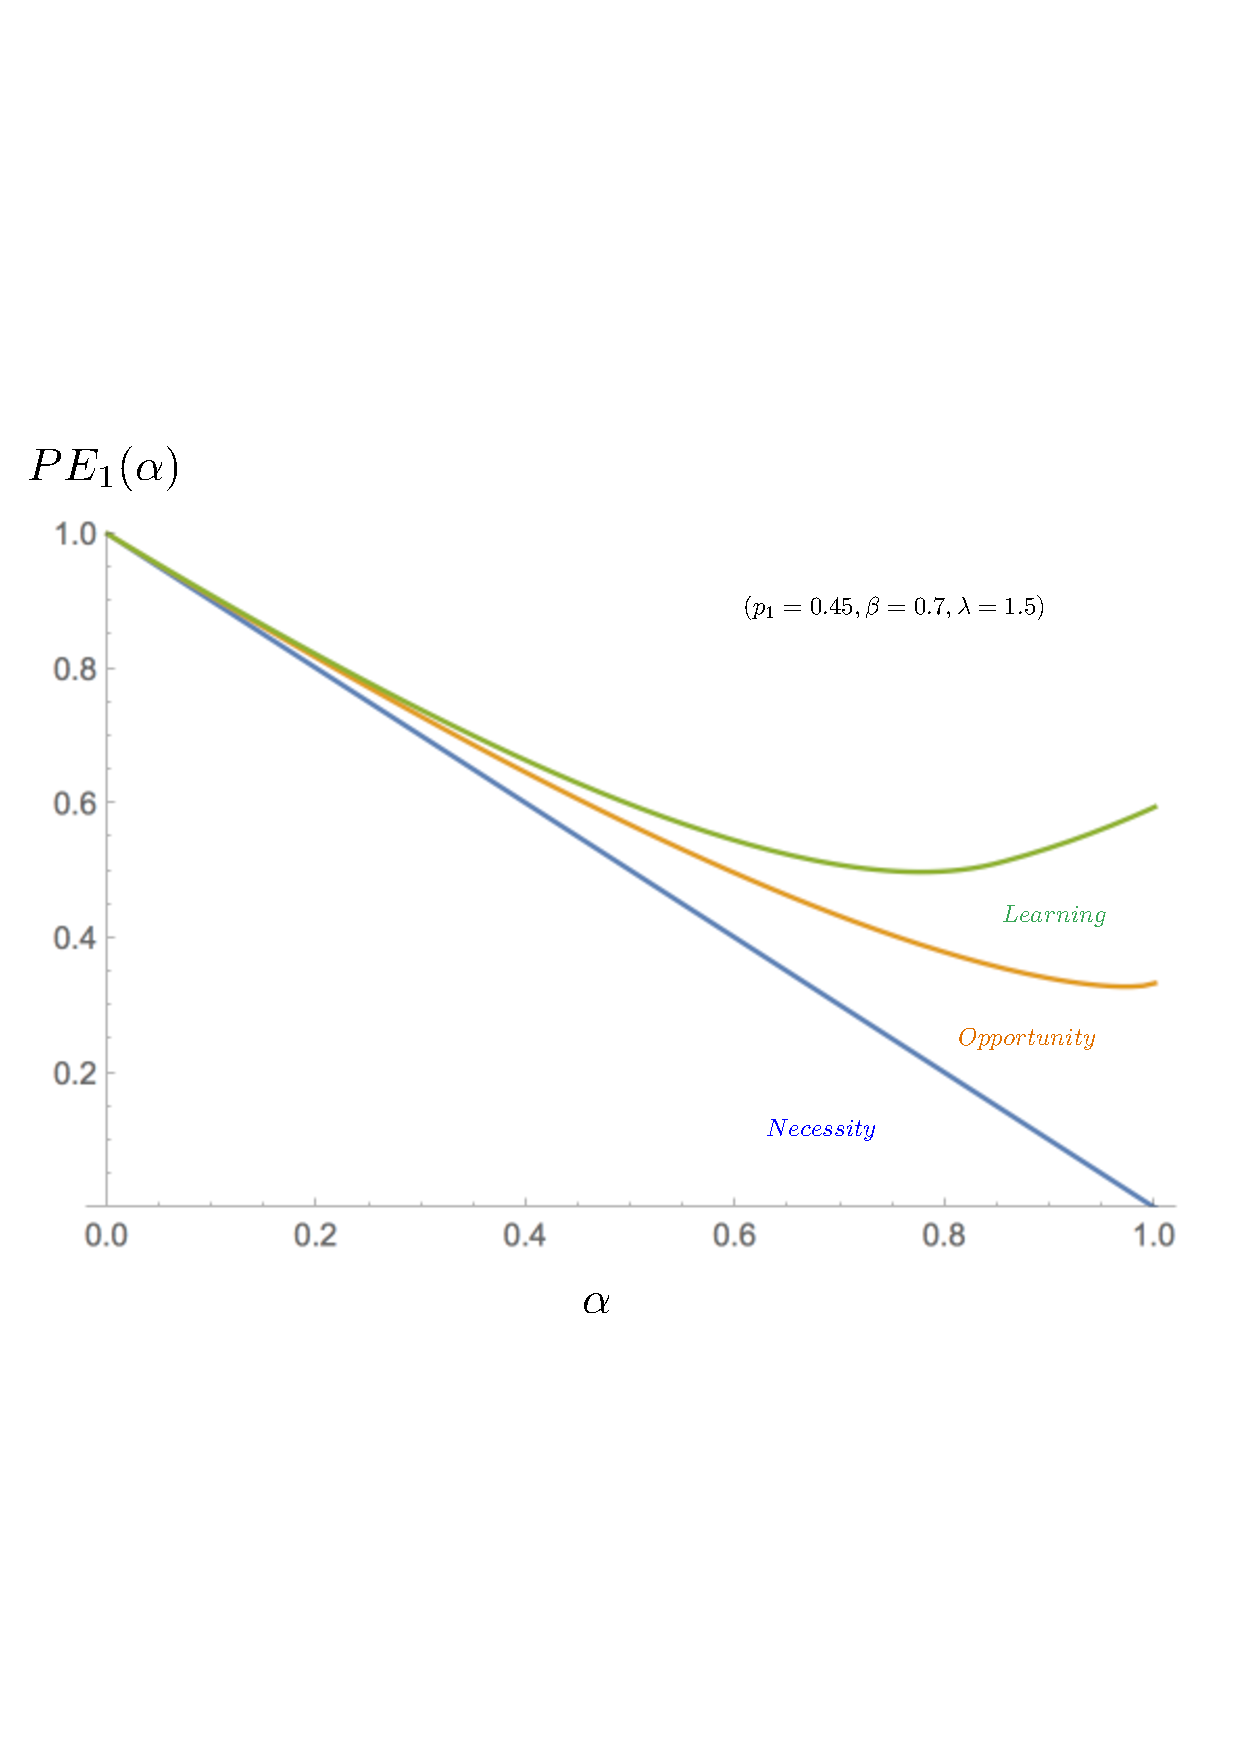
\includegraphics[scale=0.5]{proba-entrepreneur-labels}
\end{figure}

\end{frame}
%%%%%%%%%%%%%%%%%%%%%%%%%%%%%%%%%%%%%%%%
\begin{frame}
	\frametitle{}
	
\begin{lemma}
$P_1^E(\alpha)-P_2^E(\alpha)$ is negative for $\alpha$ sufficiently low and positive for $\alpha$ sufficiently high.
\end{lemma}

\begin{block}{Proposition}
 The probabilities of serial entrepreneurs and the average probability of entrepreneurs are decreasing for $\alpha$ close to 0, and increasing for $\alpha$ close to 1 if 
\begin{equation}\label{eq: prop 4}
\frac{ \sigma_2(A)- \sigma_2(B)}{ \sigma_1(B)- \sigma_1(A)}>\frac{4 \lambda^2 (1-\beta)}{\lambda -1}
\end{equation}
\end{block}

\end{frame}
%%%%%%%%%%%%%%%%%%%%%%%%%%%%%%%%%%%%%%%%
\begin{frame}
	\frametitle{Past Failures and Future Successes}
\begin{block}{Proposition}
	For a serial entrepreneur, the probability of succeeding as an entrepreneur in period 2 is increasing in $\alpha$. Furthermore
 \begin{itemize}\setlength\itemsep{0em}
\item If talent is vertical, failures are always ``bad news''. That is, the probability of succeeding in period 2 as an entrepreneur following an entrepreneurial failure in period 1 is below the initial probability of success $\sigma_1 (B)$ for all $\alpha$. 
\item If talent is horizontal, $\lambda$ is close to 1 and  $p_1<q_B$, there exists a $\bar \alpha$ such that failures are good news for $\alpha>\bar \alpha$  but bad news for $\alpha< \bar \alpha$.
\end{itemize}
\end{block}

\vspace{0.5cm}
\textcolor{gray}{$\rightarrow$ Gompers et al. 2010 vs Gottschalk et al. 2014.}
\end{frame}
%%%%%%%%%%%%%%%%%%%%%%%%%%%%%%%%%%%%%%%%
\section{conclusion}
\begin{frame}
	\frametitle{Conclusion}
Well functioning labor markets make firms  short-termists, create a learning motive for entrepreneurs, may increase their future probability of success or give them a wage premium  if they go back to employment.
%disucss US vs EU (arrival rate of offers)
\pause
\begin{itemize}[<+->]
	\item \structure{Financial frictions:} if frictionless labor market, firms competition for workers lead them to be short-termists. Otherwise complement labor market frictions
	\item \structure{Learning by doing:} agents are not able to increase their productivity. Results hold if this effect is small enough.
	\item \structure{Long-term contracting:} weakens but does not negate results
	\item \structure{Task-discretion:} should expect more of it in the EU regime since firms more willing to experiment. (OECD 2013 study)
	\item \structure{Multiple tasks:} Lazear (2004); entrepreneurs have a more ``balanced set of skills''.
	\end{itemize}

\end{frame}
%%%%%%%%%%%%%%%%%%%%%%%%%%%%%%%%%%%%%%%%
%%%%%
%   
% Appendix: conditions for informativeness of A ‰               
%    
%%%%%
\section{appendix}
\begin{frame}[label=mps]
	\frametitle{}
\begin{proposition}\label{prop:nsc_learning_vertical}
In the vertical talent case there is a conflict between maximizing today's probability of success and tomorrow's if and only if $p_1>q_A$.
\end{proposition}
%
%
\begin{proposition}\label{prop:nsc_learning_horizonthal}
In the horizontal talent case there is a conflict between maximizing today's probability of success and tomorrow's if:
\begin{align*}
p_1>q_A \;\;\mbox{and}\;\;h_A-l_A>l_B \cdot h_A-l_A \cdot h_B >l_B-h_B.
\end{align*}
\end{proposition}

\hyperlink{sigma2<5>}{\beamerreturnbutton{Back}}
\end{frame}

%%%%%%%%%%%%%%%%%%%%%%%%%%%%%%%%%%%%%%%%
\end{document} 